\documentclass[11pt]{article}

\usepackage[a4paper,margin=25mm]{geometry}
\usepackage{amsmath,amssymb,amsthm}
\usepackage{booktabs}
\usepackage{graphicx}
\usepackage{microtype}
\usepackage{xcolor}
\usepackage{enumitem}
\usepackage{hyperref}
\usepackage{cleveref}

\hypersetup{colorlinks=true,linkcolor=blue!55!black,citecolor=blue!55!black,
  urlcolor=blue!55!black,
  pdftitle={Fail-Closed Gradient-to-QEF Contracts for Approximate Implicit CSG},
  pdfauthor={Jeremy Pei},
  pdfkeywords={implicit surfaces, signed distance fields, constructive solid geometry, Dual Contouring, Hermite data, quadratic error functions, verified geometry}}
\newtheorem{theorem}{Theorem}
\newtheorem{proposition}[theorem]{Proposition}
\newtheorem{lemma}[theorem]{Lemma}
\newtheorem{corollary}[theorem]{Corollary}
\theoremstyle{definition}
\newtheorem{definition}[theorem]{Definition}
\newtheorem{remark}[theorem]{Remark}

\newcommand{\R}{\mathbb{R}}
\newcommand{\norm}[1]{\left\lVert#1\right\rVert}
\newcommand{\Certified}{\textsc{Certified}}
\newcommand{\Unknown}{\textsc{Unknown}}
\newcommand{\Invalid}{\textsc{Invalid}}

\title{Fail-Closed Gradient-to-QEF Contracts for Approximate Implicit CSG}
\author{Jeremy Pei\thanks{Corresponding author: \href{mailto:jypei@tutamail.com}{jypei@tutamail.com}}\\
Independent Researcher, Changzhou, Jiangsu, China\\
\href{https://orcid.org/0000-0002-0201-6255}{ORCID: 0000-0002-0201-6255}}
\date{}

\begin{document}
\maketitle

\begin{abstract}
Dual Contouring places one vertex per active cell by minimizing a quadratic
error function (QEF) assembled from Hermite points and normals.  For an
approximate implicit CSG field, however, a small value error does not by itself
stabilize the active Boolean branch, the normal, the edge intersection, or the
QEF solution.  We develop a local, fail-closed contract that connects these
quantities.  First, a differentiable half-space construction shows that,
without a positive branch margin, value errors tending to zero can still cause
a fixed normal jump at a hard Boolean switch.  A positive result therefore
propagates a single-normal contract only on branch-separated cells; unresolved
switch cells carry a set-valued normal enclosure or return \Unknown.  For a
binary log-sum-exp smooth minimum, we derive an executable gradient bound that
contains an unavoidable coupling from value error to weight and gradient
error.  We then transfer a field-value budget and directional-derivative lower
bound to an edge-root displacement, normalize a gradient contract into a
normal bound, and obtain a local Hermite-plane budget.  Finally, an
observed-side spectral guard and Weyl perturbation yield an absolute
displacement bound for a regularized QEF vertex.  An executable audit checks
250,000 smooth-Boolean cases, 30,000 nonlinear edge roots, and 60,000 QEF
systems with no violation of the complete bounds.  The QEF audit includes
20,000 non-concurrent systems: inconsistent analytic planes and Hermite
patches sampled from spheres and paraboloids.  Omitting the smooth
value--gradient coupling causes 31,479 failures; omitting the Hermite point
budget causes 2,874 QEF-bound failures across the two QEF audits.  In the
original 40,000-system conditioning audit, regularization makes every bound
finite, while a geometry-only identifiability guard is positive in 50.99\%.
Only 17.42\% meet a strict one-percent-of-cell tolerance,
exposing the conservatism of a worst-case certificate.  At a tolerance of
0.10 cell units, deployable coverage is 46.75\%; replacing declared budgets by
realized errors raises the diagnostic coverage to 53.52\%, while using exact
matrix perturbations raises it to 76.32\%.  Thus both input-contract width and
analytical aggregation contribute to the slack.  At \(\tau=0.10\), measured
displacement is within tolerance in 99.8475\% of those 40,000 systems, showing
that the observed non-certification gap is almost entirely certificate slack.
On a frozen corpus of 528 STEP files, OpenCascade imports and validates every
solid subset; a no-healing mesh gate admits 511 models.  A standalone
regular-grid Dual Contouring pipeline completes 118 of 122 selected models and
audits 162,216 active QEF cells with zero complete-bound violations.  Its
22.73\% coverage is explicitly oracle-diagnostic because the CAD files do not
provide certified upstream value and gradient budgets.
The result is a verifiable cell-level interface for future
certified contouring, not a claim that arbitrary sampled or neural fields
already provide the required upstream budgets.
\end{abstract}

\section{Introduction}

Signed distance fields (SDFs) support compact Boolean modeling and simple
surface interrogation.  Their numerical approximations are commonly consumed
by contouring algorithms as if the value, gradient, projected surface point,
and local tangent plane were mutually consistent.  This assumption is fragile
after approximation and CSG composition.  A hard minimum can switch its active
operand under an arbitrarily small value perturbation.  A smooth minimum avoids
non-differentiability, but the interpolation weights depend on the uncertain
values and therefore transfer value error into gradient error.  Even a bounded
normal error does not bound a QEF vertex unless the Hermite point locations and
the linear-system conditioning are controlled as well.

The original Dual Contouring method assumes Hermite data consisting of exact
intersections and normals~\cite{ju2002dual}.  It recognizes that noisy,
nearly-coplanar normals make the QEF nearly singular and uses experimentally
chosen singular-value truncation.  Later work models point and normal noise
probabilistically~\cite{trettner2020probabilistic}, or avoids arbitrary gradient
access when reconstructing from sampled SDF data~\cite{carrera2026dual}.
Recent SDF contouring also estimates gradients and filters unreliable contact
points~\cite{kohlbrenner2026gradients}.  These methods address important
reconstruction and robustness questions, but they do not provide the
worst-case compositional contract studied here: given explicit upstream value
and gradient budgets for a CSG cell, decide whether a particular Hermite/QEF
query has a checkable error bound.

Several neighboring lines of work certify different objects.  Distance-estimate
analysis tracks value or tracing precision through CSG operations
\cite{balint2023sdfe}; Lipschitz pruning identifies a regionally equivalent
subtree without propagating derivative uncertainty~\cite{barbier2025pruning};
and differentiable Boolean operators are designed for continuous optimization
rather than worst-case certification~\cite{liu2024fuzzy}.  Producer-side work
such as HotSpot improves the distance semantics of learned fields
\cite{wang2025hotspot}.  These results strengthen the motivation for explicit
contracts, but they do not by themselves transfer bounded value and gradient
uncertainty to a per-cell Hermite-plane and regularized-QEF displacement bound.

We make six contributions.

\begin{enumerate}[leftmargin=*,itemsep=2pt]
\item We prove that hard Boolean fields have no uniform,
branch-independent single-normal continuity near a switch, even when the input
gradient errors are zero and the value errors tend to zero.
\item We replace a nonexistent global single-normal rule by two sound cases:
branch-separated inheritance and a set-valued normal enclosure on unresolved
switch cells.
\item We derive a binary smooth-min gradient bound with a computable
value--gradient coupling term.
\item We prove a contract chain from an edge-root budget through a normalized
normal and local Hermite plane to an observed-side regularized QEF bound.
\item We provide a deterministic, frozen audit with two falsifying ablations,
and report both soundness evidence and certificate conservatism.
\item We quantify where the certificate is useful rather than reporting
soundness alone.  At tolerance \(\tau=0.10\), deployable coverage ranges from
98.31\% on orthogonal systems to 9.33\% on the \(20^\circ\) edge systems.  A
separate 20,000-case residual-stress audit covers non-concurrent analytic
planes and sphere/paraboloid Hermite patches.
\item We execute a frozen 528-model STEP/B-rep preflight and a 122-model
regular-grid Dual Contouring audit.  The experiment preserves every rejection
in the denominator, cross-checks OpenCascade through a second frontend and
version, and separates measured oracle diagnostics from deployable contracts.
\end{enumerate}

Our scope is intentionally local.  We do not claim a certificate producer for
arbitrary neural fields, a crack-free adaptive octree theorem, or a complete
composition theorem for deep CSG trees mixing union, intersection, and
difference.  The real-CAD implementation is a uniform-grid experimental
pipeline, not a production adaptive contourer.

\section{Related work}

\paragraph{Hermite contouring and QEFs.}
Extended Marching Cubes and Dual Contouring use surface intersections and
normals to preserve sharp features.  Ju et al.~\cite{ju2002dual} express a
cell's QEF as

\[
E(x)=\sum_i(n_i^\top(x-p_i))^2=\norm{Nx-h}_2^2,
\]

and discuss QR representation and SVD truncation for numerical robustness.
Their thresholding rule handles rank deficiency in practice but does not
certify the output under bounded perturbations of the Hermite inputs.
Probabilistic Quadrics~\cite{trettner2020probabilistic} instead minimize an
expected error under Gaussian point and normal distributions.  That work is a
principled uncertainty model and prevents us from describing all previous
QEF treatment as heuristic.  Our distinction is logical and statistical:
we propagate deterministic worst-case sets and return \Unknown when their
worst case cannot be certified; probabilistic quadrics optimize an expected
quadratic error under a chosen distribution.

Topology-oriented extensions certify complementary properties.  Manifold Dual
Contouring guarantees manifold output under adaptive simplification
\cite{schaefer2007manifold}, while interval subdivision can produce isotopic
approximations of sufficiently regular implicit surfaces
\cite{plantinga2004isotopic}.  Such connectivity and isotopy guarantees do not
bound how errors in an approximate field move a particular Hermite point,
normal, or QEF minimizer.  Conversely, the cell-level certificate developed
here does not imply a crack-free, manifold, or isotopic global mesh.

\paragraph{CSG values, activity, and differentiability.}
B\'alint et al.~\cite{balint2023sdfe} analyze signed-distance estimates under
CSG operations and quantify region-dependent precision loss.  Lipschitz
Pruning~\cite{barbier2025pruning} conservatively removes primitives that cannot
affect a spatial region and supports hard and smooth CSG.  Liu et
al.~\cite{liu2024fuzzy} instead make the Boolean operator differentiable with
respect to its type for inverse modeling.  These works respectively address
distance-value semantics, regional expression equivalence, and optimizable
operator design.  The present question is different: conditional on explicit
value and gradient budgets, what can a downstream Hermite/QEF consumer certify
for one query?

\paragraph{Approximate and learned fields.}
Neural Dual Contouring predicts vertices and topology directly from sampled
fields~\cite{chen2022ndc}.  DualMesh-UDF observes that neural UDF values and
gradients are unreliable near the zero set and cut locus, and estimates tangent
planes from filtered off-surface samples~\cite{zhang2023udf}.  Carrera et
al.~\cite{carrera2026dual} reconstruct sharp features from discrete SDF samples
without requiring arbitrary gradient queries.  Kohlbrenner and
Alexa~\cite{kohlbrenner2026gradients} approximate gradients from a tessellation
and filter infeasible contact points before surface reconstruction.  These
methods demonstrate that gradient acquisition is itself a substantive problem.
The present contract consumes a certified gradient enclosure; it does not
claim to manufacture one for these inputs.
HotSpot~\cite{wang2025hotspot} gives an asymptotically sufficient training
condition for convergence toward a true neural SDF.  That producer-side
guarantee is stronger than an Eikonal loss alone, but it is not a finite,
per-query value--gradient budget of the form consumed here.

\paragraph{Nonsmooth and verified geometry.}
At a hard Boolean switch, the classical gradient need not exist.  We use the
Clarke generalized gradient~\cite{clarke1990optimization} only as a safe
set-valued enclosure, not as a unique surface normal.  Interval and
isotopy-preserving implicit meshing methods~\cite{plantinga2004isotopic} show
the value of fail-closed local predicates, but our target is specifically the
transfer of field uncertainty to Hermite planes and QEF vertices.

\section{Contracts and semantics}

We use the convention that an SDF is positive outside.  A hard union is
therefore \(\min(\phi_A,\phi_B)\), and a hard intersection is the corresponding
maximum.

\begin{definition}[Local gradient field contract]
For a cell \(C\subset\R^d\), a contract for an approximate field
\(\widehat\phi\) records a value-error budget \(\varepsilon\), a set-valued
gradient enclosure \(G_C\), the value and gradient validity domains, and
certified branch information.  In the ball representation,
\[
|\widehat\phi-\phi|\le\varepsilon,
\qquad
\norm{\nabla\widehat\phi-\nabla\phi}\le g
\quad\text{on }C.
\]
\end{definition}

Every consumer returns one of three logical states.  \Certified\ means all
preconditions hold and an explicit bound is returned.  \Unknown\ means the
geometry may be valid but the available information is insufficient.
\Invalid\ means a validity domain or basic input contract was violated.  A
heuristic centroid or SVD fallback after \Unknown\ is an \emph{uncertified
fallback}; it is not silently reclassified as safe.

\section{Hard Boolean gradients}

The first result is deliberately stated at differentiability points, avoiding
the ill-posed comparison of classical gradients directly on a hard-min tie.

\begin{theorem}[No branch-independent single-normal continuity]
\label{thm:hard-negative}
Fix \(\theta\in(0,\pi]\).  In every neighborhood of the origin there are exact
half-space SDFs \(\phi_A,\phi_B\), approximate SDFs
\(\widehat\phi_A,\widehat\phi_B\), and points \(x_\varepsilon\) at which both
hard minima are differentiable, such that
\[
\norm{\widehat\phi_i-\phi_i}_\infty=\varepsilon,
\qquad
\nabla\widehat\phi_i=\nabla\phi_i,
\]
but
\[
\norm{\nabla\min(\widehat\phi_A,\widehat\phi_B)(x_\varepsilon)
-\nabla\min(\phi_A,\phi_B)(x_\varepsilon)}
=2\sin(\theta/2).
\]
\end{theorem}

\begin{proof}
Choose unit vectors \(n_A,n_B\) with angle \(\theta\), set \(d=n_B-n_A\), and
let \(\phi_i(x)=n_i^\top x\).  For \(\varepsilon>0\), define
\[
x_\varepsilon=\frac{\varepsilon}{\norm{d}^2}d,
\quad
\widehat\phi_A=\phi_A+\varepsilon,
\quad
\widehat\phi_B=\phi_B-\varepsilon.
\]
Then
\(
\phi_B(x_\varepsilon)-\phi_A(x_\varepsilon)=\varepsilon>0
\), so the exact minimum uniquely selects \(A\).  The approximate gap is
\(
\widehat\phi_B-\widehat\phi_A=-\varepsilon<0
\), so the approximate minimum uniquely selects \(B\).  The two gradients are
therefore \(n_A\) and \(n_B\), whose distance is
\(
\sqrt{2-2\cos\theta}=2\sin(\theta/2)
\).  Finally \(x_\varepsilon\to0\), while every \(x_\varepsilon\) remains off
the tie.
\end{proof}

The result does not say that hard Boolean gradient information is impossible.
It identifies the missing precondition.

\begin{theorem}[Branch-separated inheritance]
\label{thm:branch}
Suppose \( |\widehat\phi_i-\phi_i|\le\varepsilon_i \) throughout \(C\), and
\[
\sup_C\widehat\phi_A+\varepsilon_A
<\inf_C\widehat\phi_B-\varepsilon_B. \tag{1}
\]
Then \(\phi_A<\phi_B\) throughout \(C\).  Hence the hard union equals
\(\phi_A\) on \(C\), and every valid local value or gradient contract for
branch \(A\) transfers unchanged.
\end{theorem}

\begin{proof}
For any \(x\in C\),
\[
\phi_A(x)\le\widehat\phi_A(x)+\varepsilon_A
\le\sup_C\widehat\phi_A+\varepsilon_A,
\]
whereas
\[
\phi_B(x)\ge\widehat\phi_B(x)-\varepsilon_B
\ge\inf_C\widehat\phi_B-\varepsilon_B.
\]
Equation (1) gives the strict ordering.
\end{proof}

\begin{proposition}[Set-valued switch enclosure]
\label{prop:clarke}
If \(\phi_A,\phi_B\) are continuously differentiable near a tie \(x\), then the
Clarke generalized gradient of \(\psi=\min(\phi_A,\phi_B)\) obeys
\[
\partial_C\psi(x)
\subseteq\operatorname{conv}
\{\nabla\phi_A(x),\nabla\phi_B(x)\}.
\]
For operand enclosures \(G_A,G_B\), the convex hull
\(
\operatorname{conv}(G_A\cup G_B)
\)
is therefore a safe cell-level enclosure.
\end{proposition}

\begin{proof}
Since \(\phi_A\) and \(\phi_B\) are continuously differentiable near \(x\),
each is Clarke regular there, with
\(\partial_C\phi_i(x)=\{\nabla\phi_i(x)\}\).  For a finite pointwise minimum,
the Clarke generalized gradient is contained in the convex hull of the
generalized gradients of the active operands; at a tie both operands are
active.  The first inclusion follows.  Monotonicity of the convex hull under
set inclusion then gives the enclosure
\(\operatorname{conv}(G_A\cup G_B)\).
\end{proof}

This enclosure is not a unique normal.  Near a sharp Boolean feature, keeping
multiple constraints may be preferable to averaging them, because the QEF uses
their directional diversity to locate an edge or corner.

\section{Smooth Boolean gradient propagation}

For \(k>0\), define
\[
\psi_k(a,b)=-k\log(e^{-a/k}+e^{-b/k}),
\qquad
w_A=\frac{e^{-a/k}}{e^{-a/k}+e^{-b/k}},
\quad w_B=1-w_A.
\]
Then \(\nabla\psi_k=w_A\nabla\phi_A+w_B\nabla\phi_B\).

\begin{theorem}[Executable binary smooth-min bound]
\label{thm:smooth}
At a point \(x\), assume
\[
|\widehat\phi_i-\phi_i|\le\varepsilon_i,
\qquad
\norm{\nabla\widehat\phi_i-\nabla\phi_i}\le g_i.
\]
Let \(\widehat w_i\) be the weights computed from the approximate values.  If
\[
M_{AB}\ge\norm{\nabla\phi_A-\nabla\phi_B},
\]
then
\[
\norm{\nabla\widehat\psi_k-\nabla\psi_k}
\le
\widehat w_Ag_A+\widehat w_Bg_B
+\frac{\varepsilon_A+\varepsilon_B}{4k}M_{AB}. \tag{2}
\]
The executable choice
\[
M_{AB}=\norm{\nabla\widehat\phi_A-\nabla\widehat\phi_B}+g_A+g_B \tag{3}
\]
depends only on approximate gradients and their input budgets.
\end{theorem}

\begin{proof}
Adding and subtracting the true gradients under the approximate weights gives
\[
\begin{aligned}
\nabla\widehat\psi_k-\nabla\psi_k
={}&\widehat w_A(\nabla\widehat\phi_A-\nabla\phi_A)
+\widehat w_B(\nabla\widehat\phi_B-\nabla\phi_B)\\
&+(\widehat w_A-w_A)(\nabla\phi_A-\nabla\phi_B).
\end{aligned}
\]
The first line is bounded by
\(
\widehat w_Ag_A+\widehat w_Bg_B
\).  Writing \(w_A=\sigma((b-a)/k)\), the logistic derivative satisfies
\(
\sigma'(z)=\sigma(z)(1-\sigma(z))\le1/4
\).  The mean-value theorem yields
\[
|\widehat w_A-w_A|
\le\frac{\varepsilon_A+\varepsilon_B}{4k}.
\]
The triangle inequality gives (2), and a second triangle inequality gives
(3).
\end{proof}

\begin{remark}[No unit-gradient assumption]
\label{rem:no-eikonal}
The executable bound does not assume
\(\norm{\nabla\phi_A}=\norm{\nabla\phi_B}=1\).  Its proof uses only the
stated value and gradient budgets.  In particular, the choice in (3) remains
valid for non-unit true gradients because it follows directly from the
triangle inequality.
\end{remark}

The (1/k) factor is not an artifact: the operator becomes ill-conditioned as
it approaches a hard switch.  The audit in \cref{sec:experiments} explicitly
tests the tempting but unsound rule obtained by deleting the second term of
(2).

\section{Hermite contracts}

We next bridge field uncertainty to the plane constraints actually consumed by
a QEF.

\begin{theorem}[Certified edge-root displacement]
\label{thm:root}
Parameterize an edge by arc length \(s\in[0,L]\).  Suppose \(f\in C^1\) has a
root \(s_\star\) and satisfies
\[
|f'(s)|\ge m_e>0 \quad\text{on }[0,L].
\]
Let \(\norm{\widehat f-f}_\infty\le\varepsilon_\phi\), and let
\(\widehat s\in[0,L]\) satisfy
\(
|\widehat f(\widehat s)|\le\eta_{\rm solve}
\).  Then \(f\) is strictly monotone, its root is unique, and
\[
|\widehat s-s_\star|
\le\eta_p:=\frac{\varepsilon_\phi+\eta_{\rm solve}}{m_e}. \tag{4}
\]
\end{theorem}

\begin{proof}
Continuity and the positive lower bound prevent \(f'\) from changing sign.
Moreover
\(
|f(\widehat s)|\le\varepsilon_\phi+\eta_{\rm solve}
\).  The mean-value theorem between \(s_\star\) and \(\widehat s\) gives (4).
\end{proof}

A sign change alone does not imply uniqueness; the directional-derivative
lower bound is a real contract obligation.

\begin{lemma}[Normalized direction]
\label{lem:normal}
If \(\norm u\ge\mu>0\) and \(\norm{u-v}\le g<\mu\), then
\[
\norm{\frac{u}{\norm u}-\frac{v}{\norm v}}
\le\frac{\sqrt{2}\,g}{\mu}=: \eta_n. \tag{5}
\]
\end{lemma}

\begin{proof}
Let \(\alpha\in[0,\pi]\) be the angle between \(u\) and \(v\), so that
\(
\norm{u/\norm u-v/\norm v}=2\sin(\alpha/2)
\).
The point \(v\) lies in the closed ball of radius \(g\) about \(u\).  Since
\(g<\norm u\), this ball excludes the origin, and its angular radius as seen
from the origin is \(\arcsin(g/\norm u)\).  Hence
\(\alpha\le\arcsin t\), where
\(t:=g/\norm u\le g/\mu<1\).  The half-angle identity gives
\[
2\sin\!\left(\tfrac12\arcsin t\right)
=\sqrt{2\left(1-\sqrt{1-t^2}\right)}.
\]
The ratio
\[
F(t):=\frac{\sqrt{2(1-\sqrt{1-t^2})}}{t}
\]
increases from \(1\) to \(\sqrt{2}\) on \((0,1)\).  Therefore
\(
\norm{u/\norm u-v/\norm v}
\le\sqrt{2}\,t\le\sqrt{2}\,g/\mu
\).
\end{proof}

Let \(c\) be the cell center, and write a local Hermite plane as
\(
n^\top y=h
\), where \(y=x-c\) and \(h=n^\top(p-c)\).

\begin{lemma}[Local plane offset]
\label{lem:plane}
If
\[
\norm{p-c}\le R_c,
\quad\norm{\widehat p-p}\le\eta_p,
\quad\norm{\widehat n-n}\le\eta_n,
\]
and both normals are unit length, then
\[
|\widehat h-h|\le\eta_p+R_c\eta_n=: \eta_h^{\rm loc}. \tag{6}
\]
\end{lemma}

\begin{proof}
Expand
\[
\widehat h-h
=(\widehat n-n)^\top(p-c)
+\widehat n^\top(\widehat p-p)
\]
and apply Cauchy--Schwarz.
\end{proof}

Centering the coordinate system at the cell makes the bound invariant under a
global translation and keeps it proportional to cell scale.

\section{Observed-side regularized QEF certificate}

Stack \(m\) unit normals as rows of \(N\in\R^{m\times d}\) and the local plane
offsets into \(h\in\R^m\).  We analyze
\[
\min_y\norm{Ny-h}_2^2+\lambda\norm y_2^2,
\quad
H=N^\top N+\lambda I,
\quad q=N^\top h. \tag{7}
\]
The regularization provides a controlled fallback from exact feature
intersection to a strongly convex cell objective.  Unregularized rank-truncated
QEFs require a separate certified rank-selection argument.

Suppose the Hermite contracts give row-wise budgets
\[
\norm{n_i-\widehat n_i}\le\eta_{n,i},
\qquad
|h_i-\widehat h_i|\le\eta_{h,i},
\]
and set
\[
\eta_N=\left(\sum_i\eta_{n,i}^2\right)^{1/2},
\qquad
E_h=\left(\sum_i\eta_{h,i}^2\right)^{1/2}. \tag{8}
\]

\begin{lemma}[Observed perturbation budgets]
\label{lem:qef-budgets}
The quantities
\[
\eta_H=2\norm{\widehat N}_2\eta_N+\eta_N^2, \tag{9}
\]
\[
\eta_q=\norm{\widehat N}_2E_h
+\eta_N\norm{\widehat h}_2+\eta_NE_h \tag{10}
\]
satisfy
\(
\norm{H-\widehat H}_2\le\eta_H
\) and
\(
\norm{q-\widehat q}_2\le\eta_q
\).
\end{lemma}

\begin{proof}
Let \(E=N-\widehat N\) and \(e=h-\widehat h\).  Equation (8) gives
\(
\norm E_2\le\norm E_F\le\eta_N
\) and \(\norm e_2\le E_h\).  Expand
\[
H-\widehat H
=\widehat N^\top E+E^\top\widehat N+E^\top E
\]
and
\[
q-\widehat q
=\widehat N^\top e+E^\top\widehat h+E^\top e.
\]
Submultiplicativity gives (9)--(10).
\end{proof}

\begin{remark}[Structured row certificates]
\label{rem:row-structure}
The aggregation in (8) is deliberately worst case:
\(\norm E_2\le\norm E_F\le\eta_N\).  A smaller realized value of
\(\norm{N-\widehat N}_2\) is not deployable because the true matrix \(N\) is
unknown.  If an upstream producer can instead certify a computable
operator-norm budget \(\eta_N^{\rm op}\ge\norm E_2\), then
\cref{lem:qef-budgets,thm:qef} remain valid after replacing \(\eta_N\) by
\(\eta_N^{\rm op}\) in (9)--(10).  Thus exploiting cross-row structure requires
an explicit upstream certificate; an empirical oracle ratio is not a runtime
guard.
\end{remark}

\begin{theorem}[Certified regularized QEF displacement]
\label{thm:qef}
Let \(\lambda\ge0\), and let \(\widehat y\) solve
\(
\widehat H\widehat y=\widehat q
\), and define the computable lower bound
\[
\underline\gamma
:=\max\{\lambda,\lambda_{\min}(\widehat H)-\eta_H\}.
\tag{11}\label{eq:qef-guard}
\]
If \(\underline\gamma>0\), then \(H\) is positive definite and the true
solution \(y\) satisfies
\[
\boxed{
\norm{\widehat y-y}_2
\le
\frac{\eta_H\norm{\widehat y}_2+\eta_q}{\underline\gamma}.}
\tag{12}\label{eq:qef-bound}
\]
\end{theorem}

\begin{proof}
Because \(H=N^\top N+\lambda I\), we have
\(\lambda_{\min}(H)\ge\lambda\).  Weyl's inequality~\cite{bhatia1997matrix}
and
\cref{lem:qef-budgets} also give
\[
\lambda_{\min}(H)
\ge\lambda_{\min}(\widehat H)-\norm{H-\widehat H}_2
\ge\lambda_{\min}(\widehat H)-\eta_H.
\]
Taking the larger lower bound gives
\(\lambda_{\min}(H)\ge\underline\gamma>0\), and hence
\(\norm{H^{-1}}_2\le1/\underline\gamma\).  Using
\(Hy=q\) and \(\widehat H\widehat y=\widehat q\),
\[
H(\widehat y-y)
=(H-\widehat H)\widehat y+(\widehat q-q).
\]
Taking norms proves (12).
\end{proof}

\begin{remark}[Well-posedness versus useful certification]
\label{rem:fail-closed}
For \(\lambda>0\), \(\underline\gamma\ge\lambda>0\), so the QEF
well-posedness test in \eqref{eq:qef-guard} alone does not produce
\Unknown.  This does not make the full consumer unconditional: validity
domains, Boolean branch state, edge-root and normal preconditions must still
pass, and the vertex is \Certified\ at tolerance \(\tau\) only when the
right-hand side of \eqref{eq:qef-bound} is at most \(\tau\).  A finite but
larger bound produces \Unknown; any centroid or other heuristic used
afterwards remains an explicitly uncertified fallback.
\end{remark}

The lower bound (11) and displacement bound (12) depend on the observed
approximate matrix and upstream budgets, not on an unknown true condition
number.  For \(\lambda>0\), (11) is always positive; if the data term is nearly
singular, it falls back to \(\lambda\) and the resulting displacement bound may
be very loose.  For \(\lambda=0\), a positive observed spectral gap is required.
A consumer requiring tolerance \(\tau\) accepts the vertex only when the
right-hand side of (12) is at most \(\tau\).

\begin{remark}[Why a direct Neumann substitution does not tighten the guard]
\label{rem:neumann}
Suppose first that \(\widehat H\) is positive definite and
\(\norm{\widehat H^{-1}}_2\eta_H<1\), equivalently
\(\eta_H<\lambda_{\min}(\widehat H)\).  The standard Neumann-series estimate
then gives
\[
\norm{H^{-1}}_2
\le
\frac{\norm{\widehat H^{-1}}_2}
{1-\norm{\widehat H^{-1}}_2\eta_H}
=\frac{1}{\lambda_{\min}(\widehat H)-\eta_H}.
\]
This is exactly the inverse of the observed spectral term already present in
(11).  Because \(\underline\gamma\) is the maximum of that term and
\(\lambda\), we have
\[
\frac{1}{\underline\gamma}
\le
\frac{1}{\lambda_{\min}(\widehat H)-\eta_H}.
\]
Thus a direct Neumann substitution, with the same perturbation budgets and
numerator, cannot tighten (12).  When the Neumann condition fails, it provides
no finite inverse estimate, whereas \(\lambda>0\) still yields
\(\underline\gamma\ge\lambda\).  A tighter certificate must therefore exploit
additional structure in the row perturbations or reduce the upstream budgets,
rather than merely replacing the spectral argument.  The computable
operator-norm alternative in \cref{rem:row-structure} states what additional
information would be sufficient.
\end{remark}

\paragraph{Runtime rule.}
For each cell, the consumer performs the following steps.
\begin{enumerate}[leftmargin=*,itemsep=1pt]
\item Check value/gradient validity domains and the Boolean branch state.
\item Certify each edge root, normalized normal, and local plane offset.
\item Assemble \(\widehat N,\widehat h\) and budgets (8)--(10).
\item If \(\lambda=0\) and (11) is not positive, return \Unknown.
\item Otherwise solve the QEF and evaluate (12).  Return \Certified\ at
tolerance \(\tau\) only if the bound is at most \(\tau\); otherwise return
\Unknown\ together with the finite bound.  Any downstream fallback remains
uncertified.
\end{enumerate}

\section{Executable audit}
\label{sec:experiments}

\subsection{Protocol}

The frozen experiment uses NumPy, seed 20260808, and analytic fields or
finite-dimensional QEF systems.  The figure script reads the resulting JSON
and recomputes no experiment.  Every complete-bound experiment counts
violations independently.  Two ablations are required to fail:

\begin{enumerate}[leftmargin=*]
\item delete the value--gradient coupling term from \cref{thm:smooth};
\item propagate normal error to the QEF but omit the root-position contribution
\(\eta_p\) from the plane-offset budget (6).
\end{enumerate}

The hard-switch test uses half-space angles \(30^\circ,90^\circ,150^\circ\)
and value budgets from \(10^{-1}\) to \(10^{-10}\).  The smooth-min test samples
values, \(k\in[0.01,0.5]\), value budgets, gradient budgets, and non-unit true
gradient norms.  The Hermite test uses monotone cubic fields perturbed by a
bounded sinusoid and solves a bracketed approximate root.  The first QEF audit
uses six compatible planes sharing a common point in four normal
configurations: orthogonal, random, a \(20^\circ\) edge, and near-planar.  This
isolates conditioning but gives the unregularized data term a zero-residual
solution.  A second audit removes that restriction.  It contains 10,000 plane
systems with a controlled offset component outside the range of the normal
matrix, plus 5,000 sphere and 5,000 paraboloid Hermite patches.  Unit-cube
local coordinates, varying regularization, normal budgets, and point budgets
are used throughout.

Two nondeployable diagnostic arms separate sources of QEF slack.  The first
replaces declared row budgets by the normal and point errors that actually
occurred in each synthetic trial, while retaining the same proof formulas.
The second uses the exact matrix and right-hand-side perturbations together
with the true smallest eigenvalue.  Both arms see true quantities unavailable
to a runtime consumer; they diagnose conservatism and are not additional
certificates.

\begin{figure}[t]
\centering
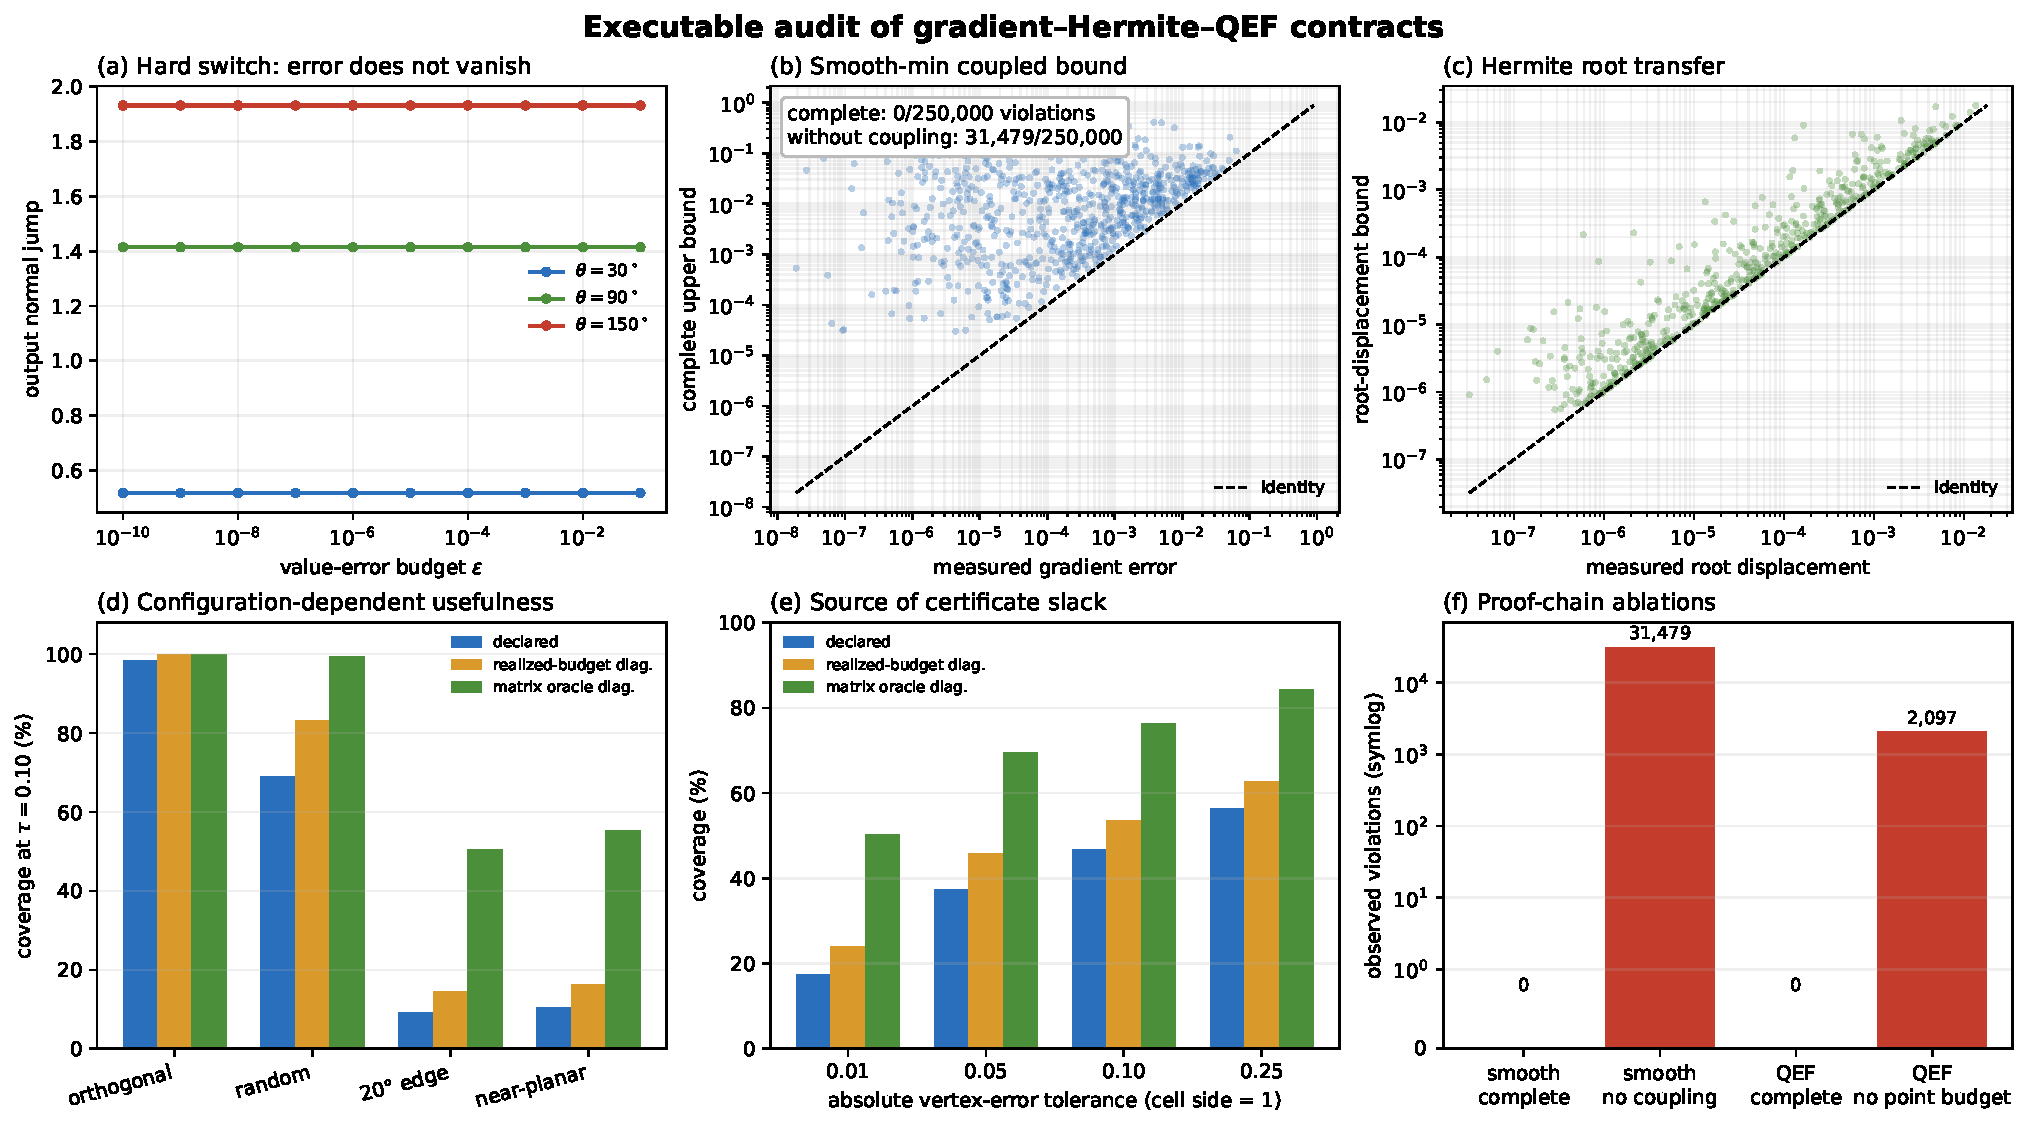
\includegraphics[width=\linewidth]{../figures/fig_topic4_contract_audit.pdf}
\caption{Executable audit.  (a) The hard-switch normal jump remains fixed as
the input value error tends to zero.  (b,c) Complete smooth-min and edge-root
bounds dominate measured errors.  (d) At \(\tau=0.10\), declared-contract
coverage is much lower on edge and near-planar configurations; realized-budget
and exact-matrix diagnostics expose where slack enters.  (e) The same three
arms are compared across tolerances.  (f) Complete bounds show zero observed
violations, while deleting the coupling or Hermite point budget yields
counterexamples.  Finite sampling validates the implementation, not the
universal theorems.}
\label{fig:audit}
\end{figure}

\subsection{Results}

\Cref{tab:summary} reports the principal counts.  The complete smooth-min and
Hermite bounds show no observed violation.  The one-sided 95\% exact lower
bounds on their finite-sample success probabilities are 99.9988\% and
99.9900\%, respectively.  These are statistical descriptions of the audit,
not replacements for the proofs.

\begin{table}[t]
\centering
\caption{Frozen executable audit.  ``Ablation failures'' count observed
violations after deleting a required proof-chain term.}
\label{tab:summary}
\resizebox{\linewidth}{!}{%
\begin{tabular}{lrrrr}
\toprule
Experiment & tested & complete-bound cases & complete failures & ablation failures\\
\midrule
Hard switch construction & 30 & 30 & 0 & --\\
Smooth-min propagation & 250,000 & 250,000 & 0 & 31,479\\
Hermite edge root & 30,000 & 30,000 & 0 & --\\
Regularized QEF & 40,000 & 40,000 & 0 & 2,097\\
Non-concurrent QEF stress & 20,000 & 20,000 & 0 & 777\\
\bottomrule
\end{tabular}
}
\end{table}

For QEFs, all 40,000 regularized systems have a finite bound and show zero
observed violations; the one-sided 95\% lower confidence bound on this finite
success proportion is 99.9925\%.  In 20,396 systems (50.99\%), the observed
data matrix itself has a certified positive spectral margin after subtracting
the perturbation budget.  This geometry-only identifiability is highly
configuration dependent (\cref{tab:qef}): it holds for almost all orthogonal
and random systems, for none of the exact two-normal edge systems, and for only
4.85\% of near-planar systems.  The regularizer still supplies a finite lower
bound in the remaining cases, but the certificate is then usually loose.

\begin{table}[t]
\centering
\caption{Configuration-wise QEF usefulness and diagnostic decomposition.
``Realized'' uses the errors that occurred in each trial; ``matrix'' uses exact
matrix perturbations and the true spectral denominator.  Both are
nondeployable diagnostics.  Coverage uses \(\tau=0.10\) cell units.}
\label{tab:qef}
\resizebox{\linewidth}{!}{%
\begin{tabular}{lrrrrrr}
\toprule
Configuration & data ID & median actual & declared & realized & matrix & declared coverage\\
\midrule
Orthogonal & 100.00\% & 0.000186 & 0.01198 & 0.00653 & 0.00139 & 98.31\%\\
Random & 99.11\% & 0.000245 & 0.04317 & 0.02324 & 0.00397 & 68.98\%\\
\(20^\circ\) edge & 0.00\% & 0.000972 & 1.60751 & 0.89061 & 0.09671 & 9.33\%\\
Near planar & 4.85\% & 0.001611 & 1.54401 & 0.82798 & 0.07484 & 10.38\%\\
\bottomrule
\end{tabular}
}
\end{table}

A finite worst-case bound need not be useful.  The median QEF bound is 0.1343
cell units, whereas the median measured error is 0.000592; the median
bound-to-error ratio is 484.  Requiring bounds of at most 0.01, 0.05, 0.10,
and 0.25 cell units yields total-query coverage of 17.42\%, 37.38\%, 46.75\%,
and 56.34\%.  This conservatism is a central result rather than a detail to
hide.  It motivates tighter structured perturbation bounds, adaptive
subdivision, and a cost--coverage analysis in the full system.

The diagnostics localize part of that conservatism.  Across all configurations,
the median declared, realized-budget, and exact-matrix bounds are 0.13431,
0.07074, and 0.00987 cell units.  At \(\tau=0.10\), their respective coverage
is 46.75\%, 53.52\%, and 76.32\%.  The gap between the first two columns is
attributable to unused width in the declared input contracts; the remaining
gap shows that row aggregation, triangle inequalities, and the observed-side
spectral lower bound also matter.  In the deployable arm, coverage at this
tolerance is only 9.33\% on the \(20^\circ\) edge configuration and 10.38\%
on near-planar configurations.  The current certificate therefore does not
provide useful coverage for most such cells at this tolerance, even though its
finite bounds remain sound in the audit.

\begin{remark}[Source of the observed coverage gap]
\label{rem:gap-source}
At \(\tau=0.10\), measured QEF displacement is within tolerance in 39,939 of
the 40,000 conditioning trials (99.8475\%), whereas the deployable certificate
accepts 18,700 (46.75\%).  Thus 53.0975 percentage points are audit false
negatives attributable to certificate slack, while 0.1525 percentage points
correspond to measured displacements that actually exceed the tolerance.  In
this audit, approximately 99.71\% of the non-certification gap is therefore
associated with conservatism rather than an above-tolerance measured
displacement.  At the level of global medians, the declared-to-realized and
realized-to-matrix ratios are 1.90 and 7.17.  These are descriptive ratios, not
a causal decomposition, but they indicate that analytical aggregation is the
larger source of slack in the present experiment.
\end{remark}

The residual-stress audit tests whether soundness depended on the compatible
common-point construction.  Its 20,000 complete bounds have zero observed
violations, with a one-sided 95\% all-success lower bound of 99.9850\%.
The median minimum unregularized data residual rises from numerical zero in the
compatible baseline to 0.00295 for inconsistent analytic planes and 0.02348
for curved Hermite patches (\cref{tab:residual-stress,fig:residual-stress}).
The complete bound remains sound, whereas deleting the Hermite point budget
causes 777 violations in these added systems.

\begin{table}[t]
\centering
\caption{Residual-stress extension of the QEF audit.  ``Measured'' and
``declared'' are coverage at \(\tau=0.10\).  The compatible baseline is the
original 40,000-system conditioning audit.}
\label{tab:residual-stress}
\resizebox{\linewidth}{!}{%
\begin{tabular}{lrrrrrrr}
\toprule
System class & tested & median residual & median actual & median bound & measured & declared & failures\\
\midrule
Compatible common point & 40,000 & \(1.25\!\times\!10^{-16}\) & 0.000592 & 0.13431 & 99.8475\% & 46.75\% & 0\\
Inconsistent analytic planes & 10,000 & 0.00295 & 0.000626 & 0.11977 & 99.73\% & 47.98\% & 0\\
Sphere/paraboloid patches & 10,000 & 0.02348 & 0.001339 & 0.37076 & 99.99\% & 27.86\% & 0\\
\bottomrule
\end{tabular}
}
\end{table}

\begin{figure}[t]
\centering
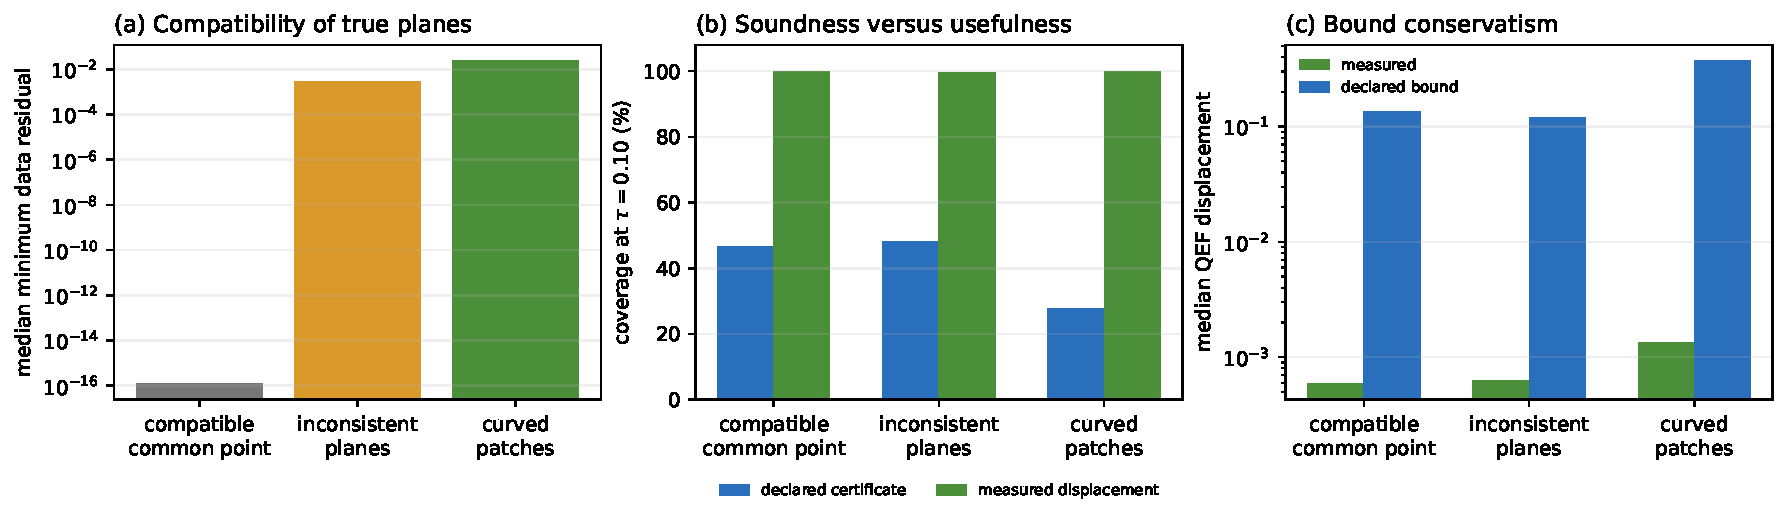
\includegraphics[width=\linewidth]{../figures/fig_topic4_residual_stress.pdf}
\caption{Audit beyond common-point Hermite systems.  (a) Inconsistent analytic
planes and curved patches have nonzero minimum data residuals.  (b) Complete
bounds remain sound, but declared coverage remains much lower than measured
within-tolerance displacement.  (c) The declared bounds remain conservative.
Finite sampling checks the implementation and does not prove the theorem.}
\label{fig:residual-stress}
\end{figure}

The ablations demonstrate that the complete chain is doing logical work.
Removing the smooth value--gradient coupling produces 31,479 failures among
250,000 tests (12.59\%).  Keeping the QEF spectral guard but omitting the
Hermite point-position budget produces 2,097 bound violations among the 40,000
compatible systems and another 777 among the 20,000 residual-stress systems.
Thus normal uncertainty alone cannot certify the QEF right-hand side.

\input{real_cad_experiment_section}

\section{Discussion}

\paragraph{Single normals versus sharp features.}
The negative result is not an argument for smoothing every Boolean crease.
At a switch, the two active normals contain useful feature information.  The
contract should preserve them as separate Hermite constraints or a normal set.
It returns \Unknown\ only when a downstream interface insists on one normal
that the upstream geometry does not uniquely define.

\paragraph{Worst case versus probabilistic uncertainty.}
The QEF bound is conservative because it assumes adversarial alignment of all
plane perturbations.  Probabilistic quadrics can be substantially more useful
when a credible distribution is available~\cite{trettner2020probabilistic}.
The two approaches answer different questions.  A promising hybrid would use
the deterministic contract as a safety envelope and a probabilistic model to
choose a high-quality point within it.

\paragraph{Regularization and bias.}
Regularization makes the QEF strongly convex and simplifies certification, but
it changes the target minimizer.  Our theorem compares approximate and true
solutions at the same \(\lambda\); it does not bound bias relative to the
unregularized surface-feature intersection.  Choosing \(\lambda\) therefore
requires a separate accuracy--conditioning tradeoff.

\paragraph{Relation to adaptive Dual Contouring.}
The current result certifies one cell's inputs and regularized QEF solution.  A
complete adaptive algorithm still needs certified active-cell detection,
consistent decisions across levels, topology or manifold conditions, and a
crack-free connectivity theorem.  The real-CAD audit implements a separate
uniform-grid Dual Contouring pipeline and exposes non-manifold connectivity on
79 of 118 completed models.  The current HybridCADLab production path still
uses Marching Cubes; the audit should therefore not be read as an adaptive or
production Dual Contouring backend.
Existing manifold and isotopy-preserving methods
\cite{schaefer2007manifold,plantinga2004isotopic} clarify the missing global
obligations, but do not eliminate the local input-uncertainty problem addressed
by the present contract.

\section{Limitations and next steps}

First, the contract consumes value and gradient budgets.  Analytic primitives
can supply them, but sampled grids and neural fields need a separate producer,
possibly based on interval interpolation, verified automatic differentiation,
or Lipschitz-constrained networks.  Empirical residuals are not automatically
valid worst-case budgets.

Second, the formal hard-Boolean result covers branch separation and a local
set-valued switch enclosure.  A deep DAG theorem must propagate validity
domains and active sets through union, intersection, and difference without
silently turning a local certificate into a global claim.

Third, the binary smooth-min bound is closed, but an (n)-ary result should use
the full softmax Jacobian rather than repeatedly applying a binary bound whose
tightness depends on tree association.

Fourth, the real-CAD arm closes the previous end-to-end implementation gap but
does not close the producer-certificate gap.  It uses a source triangle mesh
to obtain reference closest points and pseudo-normals, so its coverage is an
offline oracle diagnostic.  The uniform grid also misses four thin or
anisotropic parts at the frozen coarse resolution, and standard sign-pattern
connectivity produces non-manifold edges on many completed models.  The next
engineering stage is an adaptive, manifold-aware contourer driven by an actual
producer of certified value and gradient budgets.  A larger corpus run is
justified only after those upstream certificates execute rather than replaying
metadata or substituting empirical residuals.

Finally, the present bounds are often loose.  The current row-wise budgets
enter through the Frobenius aggregation \(\eta_N\).  A tighter deployable bound
cannot be justified from the smaller operator norm observed against an unknown
true matrix; it requires an upstream operator-norm or correlation-aware
certificate as in \cref{rem:row-structure}.  Such structured perturbation
budgets, interval eigenvalue bounds, adaptive cell subdivision, and
normal-cone-aware QEF formulations are the main routes to improve useful
coverage without weakening soundness.

\section{Conclusion}

A value-error budget is not a normal certificate, and a normal certificate is
not a QEF certificate.  The missing links are branch state, root position,
normal normalization, local plane offset, and matrix conditioning.  We have
made these links explicit in a fail-closed cell-level contract.  A hard Boolean
switch requires either certified branch separation or a set-valued normal
conclusion.  A smooth Boolean requires a value--gradient coupling term.  A QEF
requires both normal and point budgets and an observed-side spectral guard.
The analytic stress tests support the implementation and falsify two tempting
simplifications, while also showing that worst-case QEF bounds can be highly
conservative.  The added non-concurrent and curved-patch systems show that the
zero-violation result is not restricted to compatible, common-point planes.
The 528-model STEP preflight and 122-model regular-grid contouring arm further
show that the implementation runs on heterogeneous CAD geometry, while its
22.73\% oracle-diagnostic coverage and non-manifold outputs expose the remaining
producer and connectivity gaps.  Completing a production adaptive contourer is
future work; the current contribution is the theorem and software interface
that such a system must satisfy before it labels a Hermite/QEF vertex as
certified.

\section*{Reproducibility statement}

The research package contains the synthetic generator, frozen JSON record,
regression checks, figure scripts, proof-status and audit records, and this
manuscript source.  It also contains the real-CAD import and contouring source,
input receipts and hashes, row-level results, cross-version comparison,
50-to-28 selection ledger, and a fail-closed verifier with negative tamper
tests.  Third-party STEP files are not redistributed; their source records and
cryptographic hashes are provided.  The synthetic generator uses fixed seed
20260808.  Figure code reads frozen results and does not rerun experiments.  A
success message explicitly states that finite sampling is not a proof.

\section*{Conflict of interest}

The author declares no conflict of interest.

\section*{Funding}

This research received no specific grant from any funding agency in the public,
commercial, or not-for-profit sectors.

\section*{Data availability}

The source code, fixed seeds, frozen numerical results, row-level real-CAD
records, regression checks, input receipts, verification scripts, and
figure-generation scripts supporting the findings of this study are provided
as Supporting Information and in the public artifact repository
\url{https://github.com/Jeremy-Pei/gradient-qef-contracts-artifact}.  Third-party
STEP files are not redistributed; the repository provides acquisition records
and SHA-256 values so that authorized users can reconstruct and verify the
input corpus.

\section*{Ethics statement}

Ethics approval, consent to participate, and consent for publication are not
applicable because this mathematical and computational study involved no human
participants, animals, or identifiable personal data.

\section*{CRediT authorship contribution statement}

Jeremy Pei: Conceptualization; Methodology; Formal analysis; Software;
Investigation; Validation; Visualization; Writing -- original draft; Writing --
review and editing.

\section*{Declaration of generative AI and AI-assisted technologies}

During preparation of this manuscript, the author used OpenAI Codex to help
organize the research plan, draft and inspect mathematical arguments, implement
analytic stress tests, check reproducibility, and edit the language.  The
author independently reviewed and revised the mathematical arguments,
references, source code, numerical results, and wording, and takes full
responsibility for the submitted content.

\begin{thebibliography}{99}

\bibitem{ju2002dual}
T.~Ju, F.~Losasso, S.~Schaefer, J.~Warren,
Dual contouring of Hermite data,
\emph{ACM Transactions on Graphics} 21~(3) (2002) 339--346.
\href{https://doi.org/10.1145/566654.566586}{doi:10.1145/566654.566586}.

\bibitem{trettner2020probabilistic}
P.~Trettner, L.~Kobbelt,
Fast and robust QEF minimization using probabilistic quadrics,
\emph{Computer Graphics Forum} 39~(2) (2020) 325--334.
\href{https://doi.org/10.1111/cgf.13933}{doi:10.1111/cgf.13933}.

\bibitem{schaefer2007manifold}
S.~Schaefer, T.~Ju, J.~Warren,
Manifold dual contouring,
\emph{IEEE Transactions on Visualization and Computer Graphics} 13~(3)
(2007) 610--619.
\href{https://doi.org/10.1109/TVCG.2007.1012}{doi:10.1109/TVCG.2007.1012}.

\bibitem{plantinga2004isotopic}
S.~Plantinga, G.~Vegter,
Isotopic approximation of implicit curves and surfaces,
in: \emph{Symposium on Geometry Processing}, 2004, pp.~251--260.
\href{https://doi.org/10.2312/SGP/SGP04/251-260}{doi:10.2312/SGP/SGP04/251-260}.

\bibitem{chen2022ndc}
Z.~Chen, A.~Tagliasacchi, T.~Funkhouser, H.~Zhang,
Neural Dual Contouring,
\emph{ACM Transactions on Graphics} 41~(4) (2022), Article 104.
\href{https://doi.org/10.1145/3528223.3530108}{doi:10.1145/3528223.3530108}.

\bibitem{zhang2023udf}
C.~Zhang, G.~Lin, L.~Yang, X.~Li, T.~Komura, S.~Schaefer, J.~Keyser,
W.~Wang,
Surface extraction from neural unsigned distance fields,
in: \emph{Proceedings of the IEEE/CVF International Conference on Computer
Vision}, 2023.
\href{https://doi.org/10.1109/ICCV51070.2023.02059}{doi:10.1109/ICCV51070.2023.02059}.

\bibitem{wang2025hotspot}
Z.~Wang, C.~Wang, T.~Yoshino, S.~Tao, Z.~Fu, T.-M.~Li,
HotSpot: Signed distance function optimization with an asymptotically
sufficient condition,
in: \emph{Proceedings of the IEEE/CVF Conference on Computer Vision and
Pattern Recognition}, 2025, pp.~1276--1286.

\bibitem{balint2023sdfe}
C.~B\'alint, G.~Valasek, L.~Gerg\H{o},
Operations on signed distance function estimates,
\emph{Computer-Aided Design and Applications} 20~(6) (2023) 1154--1174.
\href{https://doi.org/10.14733/cadaps.2023.1154-1174}{doi:10.14733/cadaps.2023.1154-1174}.

\bibitem{barbier2025pruning}
W.~Barbier, M.~Sanchez, A.~Paris, E.~Michel, T.~Lambert, T.~Boubekeur,
M.~Paulin, T.~Thonat,
Lipschitz pruning: Hierarchical simplification of primitive-based SDFs,
\emph{Computer Graphics Forum} 44~(2) (2025), Article e70057.
\href{https://doi.org/10.1111/cgf.70057}{doi:10.1111/cgf.70057}.

\bibitem{liu2024fuzzy}
H.-T.~D. Liu, M.~Agrawala, C.~Yuksel, T.~Omernick, V.~Misra, S.~Corazza,
M.~McGuire, V.~B. Zordan,
A unified differentiable Boolean operator with fuzzy logic,
in: \emph{ACM SIGGRAPH Conference Papers}, 2024, Article 109.
\href{https://doi.org/10.1145/3641519.3657484}{doi:10.1145/3641519.3657484}.

\bibitem{carrera2026dual}
X.~Carrera, N.~Wang, C.~Batty, O.~Stein, S.~Sell\'{a}n,
Dual Contouring of Signed Distance Data,
in: \emph{SIGGRAPH Conference Papers}, 2026, Article 38.
\href{https://doi.org/10.1145/3799902.3811116}{doi:10.1145/3799902.3811116}.

\bibitem{kohlbrenner2026gradients}
M.~Kohlbrenner, M.~Alexa,
Contouring signed distance fields by approximating gradients,
\emph{Computer Graphics Forum} (2026).
\href{https://doi.org/10.1111/cgf.70373}{doi:10.1111/cgf.70373}.

\bibitem{clarke1990optimization}
F.~H. Clarke,
\emph{Optimization and Nonsmooth Analysis},
SIAM, Philadelphia, 1990.

\bibitem{bhatia1997matrix}
R.~Bhatia,
\emph{Matrix Analysis},
Springer, New York, 1997.

\end{thebibliography}

\end{document}
